\documentclass[a4paper,11pt]{article}

\usepackage{amsmath}
\usepackage{amssymb}
\usepackage{amsfonts}
\usepackage{graphicx}
\usepackage{subcaption}
\usepackage{microtype}
\usepackage{algpseudocode, algorithm}
\PassOptionsToPackage{hyphens}{url}\usepackage{hyperref}
\usepackage{physics}
\usepackage{cleveref}
\usepackage{natbib}

\title{Efficiently downsampling inelastic cyclic stress-strain data while preserving its curvature}
\author{A Hartloper}

\begin{document}
\maketitle

\begin{abstract}
    A downsampling method for stress-strain data that uses few points to preserve curvature is proposed in this document.
    This method uses existing algorithms that satisfy a local perpendicular distance criterion within a pre-defined tolerance.
    The proposed method is then extended to preserve the global difference in energy between the original and downsampled data within a specified tolerance.
    The global energy downsampling method is particularly useful because it is directly related to the metric used in material calibration.
    Results from two datasets indicate that, with around 0.5~\% difference in energy, the downsampled data has 50--90 times less points.
    The proposed method leads to 2--5 times less points than the previous integer reduction downsampling method and also appears to give a better representation of the stress-strain data.
\end{abstract}

\section{Introduction}

The raw data (i.e., extensometer displacement, load cell force) in experiments used for material model calibration are typically sampled at 10~Hz in the EPFL test setup.
As experiments range from around a few minutes (e.g., LP1) to hours (LP5), this results in thousands to hundreds of thousands of data points for each experiment.
However, the sampled data is often denser than required to reasonably describe the stress-strain behavior of materials under the applied strain rates.
When it comes to calibrating material models, the time required is proportional to the number of data points.
Therefore, time can be saved by reducing the number of data points prior to running the calibration while maintaining the fidelity of the data.

Experience has shown that the fidelity of an experiment can be kept with around 10--100 times less points depending on the load protocol.
Calibrating the UVC model using ten load protocols \emph{without} reducing the number of points could, therefore, take weeks to a year.
A ``good'' method of reducing the number of data points, or \emph{downsampling} the data, is essential to keep the calibration time reasonable (say, on the order of hours to days per material).
The properties that define a good downsampling method in this context are now defined.

A good downsampler for inelastic, cyclic, stress-strain data of structural steels:
\begin{enumerate}
    \item samples enough points in the initial elastic region to obtain a good estimate of the initial elastic modulus,
    \item samples the upper yield point,
    \item samples all the maxima and minima in each loading cycle (i.e., the \emph{peaks} of the stress-strain graph),
    \item samples enough points to retain the fidelity of curved regions in the stress-strain graph,
    \item samples as few points as necessary in straight regions,
    \item can handle noise in the measurements,
    \item can handle different strain rates,
    \item has interpretable heuristic parameters,
    \item is easy to use.
\end{enumerate}
A method that combines different techniques to satisfy these desirable properties is developed in this document.

My initial work to downsample stress-strain data combined two techniques: (i) find the peaks of the stress-strain data, then (ii) downsample by an integer factor\footnote{\url{https://en.wikipedia.org/wiki/Downsampling_(signal_processing)}}.
This method preserves the peaks, however, it either removes too many points in the curved regions, or is inefficient in the straight regions.
Moreover, it is a matter of ``art'' to pick a reasonable integer factor for each case, and, this has to be done twice for each experiment because of the different strain rates in most load protocols!
There are several areas to improve this method that lead to this study.

The initial inspiration for improvement was this blog\footnote{\label{fn:blog}\url{https://kaushikghose.wordpress.com/2017/11/25/adaptively-downsampling-a-curve/}. \hfill}.
Then I found a wealth of literature, particularly in the domain of cartography.
Two subproblems are defined in the literature related to this problem \citep{ImaiPolygonalApproximationsCurve1988}: the min-\# problem and the min-$\epsilon$ problem.
The objective of the first problem is to determined the minimum number of sample points to provide a reasonably good approximation of the curve, the second is to find the minimum error between the original and sampled curves for a given number of points.
In the first, an error critieria is specified ($\epsilon$), and in the second the number of points is specified ($N$).
Many approximate solutions exist \citep{Rameriterativeprocedurepolygonal1972,DouglasAlgorithmsreductionnumber1973,HeckbertSurveyPolygonalSurface1997} as well as optimal ones \citep{ImaiPolygonalApproximationsCurve1988,PerezOptimumpolygonalapproximation1994,ChanApproximationPolygonalCurves1996}.
The optimal solution to the first problem is easier (takes less computational effort) than the second one by a factor of $\log N$ \citep{ChanApproximationPolygonalCurves1996}.
I have focused on applications of approximate solutions to the min-\# problem.

The most popular algorithm to determine an approximate solution to the min-\# problem appears to be the Ramer–Douglas–Peucker (RDP) algorithm \citep{Rameriterativeprocedurepolygonal1972,DouglasAlgorithmsreductionnumber1973,HeckbertSurveyPolygonalSurface1997}.
The RDP algorithm is not optimal and only finds a number of points $N$ close to the minimum.
A number of additional points are certain to be added due to the criteria of selecting sample points in the algorithm.
This point will be explained later in this document.
However, the RDP algorithm is still quite good, comparatively fast, and has been widely implemented.
Excellent visualizations of the RDP algorithm can also be found\footnote{\url{https://karthaus.nl/rdp/}}\footnote{\url{https://en.wikipedia.org/wiki/Ramer-Douglas-Peucker_algorithm}}.

The aim in this document is to use these established downsampling techniques to improve upon my existing integer reduction method.
Ideally, the proposed method will be able to satisfy the desirable criteria set forth above.
The following sections outline the development process and the evaluation of the proposed method.

\section{Proposed method}

The proposed method is composed of two main parts and two auxiliary parts.
The first main part is to find the peaks in the stress-strain data.
The second main part is to downsample the entire stress-strain history based on its curvature.
The auxiliary parts are to keep additional points in the initial elastic region and remove cycles after saturation in constant amplitude tests.
The final downsampled data is the unique set of sample points from all the parts.

Mosts of the heavy lifting is done in the second main part.
The first main part is essential to overcome \emph{aliasing} in the sampled data and determine properties such as the number of cycles.
The auxiliary parts ensure fidelity of the initial elastic region and remove data that does not contribute much to the material behavior.
Details are given for each part and a summary of the entire procedure is given afterwards.

\subsection{Identifying peaks in the stress-strain graph}

The peaks in the stress-strain graph are identified by the minima or maxima in each cycle.
Cycles can be fairly reliably identified by the switching of signs in the stress signal.
Therefore, the peaks are the minima and maxima between each change in sign of the stress signal.
This method works well if the stress crosses zero in each cycle and there is no substantial noise in the stress signal around zero.

An attempt at identifying upper yield point, if it exists, is made in this first part.
First, the 0.2~\% offset yield stress is computed using the initial elastic modulus.
The initial elastic modulus itself is computed using linear regression up to $0.65 f_{y,n}$, where $f_{y,n}$ is the nominal yield stress of the material.
Then, the upper yield point is selected as the point of maximum stress up to the 0.2~\% offset yield stress.
If there is no upper yield point (due to the material or imperfections in the specimen), then the maximum will typically be at the 0.2~\% offset yield stress, and this point is sampled instead.
The upper yield point is the first ``peak'' in the stress-strain graph.

Another important point in stress-strain data tested according to the RESSLab protocols is the first instance 2~\% strain amplitude is crossed.
This point is important because the strain rate changes by a factor of around 30 after 2~\% strain.
Therefore, this point is sampled as well.
A final point is also sampled.
Unless otherwise specified (i.e., due to buckling), the final point is selected at 12.5~\% strain due to limitations in the small extensometer used for M8 experiments, or the last point in the history if 12.5~\% strain is never obtained.
Any data past the final point are neglected.

To summarize, the sampled points from the first part are:
\begin{itemize}
    \item the upper yield point (or 0.2~\% offset yield stress point),
    \item the point where 2~\% strain amplitude is crossed (not applicable for LPs~4 and~5),
    \item the peaks in the stress-strain graph, and
    \item the final point.
\end{itemize}

\subsection{Curvature-preserving downsampling}

We are concerned with preserving the ``large-scale'' curvature in a stress-strain graph, not localized curvature due to noisy measurements.
The idea in the second part of the overall procedure is to remove as many points as possible in the ``straight'' regions of the stress-strain graph and keep as many as necessary in the ``curved'' regions.
The key to these methods is to define what is ``straight'', and to sample a point every time that this condition is violated.

\subsubsection{First attempt: Maximum deivation downsampler}

The method, named the ``maximum deviation downsampler'', is outlined in Algorithm~\ref{alg:max-dev-downsampler} based on a blog by Kaushik Ghose in \cref{fn:blog}.
After further reading I realized the link with other methods outlined in the introduction.
This method requires a set of points and a tolerance, $\epsilon$.
The algorithm starts at the first point and steps forward through each point in the set.
A line is computed between the starting point and the current point.
The perpendicular distance is computed between the line and each point in the range of the starting and current point.
Therefore, the perpendicular distance acts as a proxy for the radius of curvature.
If the perpendicular distance is greater than the tolerance, the point before the current point is sampled; the sampled point is then set as the starting point and the process continues.

The keys to making Algorithm~\ref{alg:max-dev-downsampler} in the current context are to: compute an appropriate perpendicular distance, to use an appropriate tolerance, and to remove noise from the data.
One challenge in stress-strain data is that the ``distances'' in stress and strain have different units.
This is handled by normalizing the stress data by the range in stress ($\sigma_i^* = \sigma_i / (\max \sigma - \min \sigma)$), and the strain by the range in strain ($\varepsilon_i^* = \varepsilon_i / (\max \varepsilon - \min \varepsilon)$).
Therefore, the normalized values have a range of 1.0 in both axes.

Given this normalization, a tolerance of $\epsilon = 0.001$ is usually appropriate.
This tolerance can be interpreted that ``straight'' is defined as a deviation less than 1/1000'th of the maximum ``distance'' spanned by the graph.
Finally, noise in the data can cause spurious sampling of points.
Therefore, a moving average filter (Savitzky-Golay, \texttt{scipy.signal.savgol\_filter}) is applied to the stress-strain data prior to normalization.
The moving average filter requires a window length, $w$ and an interpolation order, $p$.
Filtering the stress-strain data removes the noise, but leads to aliasing.
Recall that the peaks of the stress-strain signal are already included in part 1 of the overall procedure, therefore, minor aliasing is not an issue in part 2.
Therefore, the set of 2-D points $\{x_i\}$ input to Algorithm~\ref{alg:max-dev-downsampler} are the filtered, normalized stress-strain data.

\begin{algorithm}
	\caption{Maximum deviation downsampler.}
	\label{alg:max-dev-downsampler}
	\begin{algorithmic}[1]
		\State \textbf{input:} Set of points, $\{x_i\}_{i=0}^{N-1}$ with $x_i \in \mathbb{R}^n$ and $N \in \mathbb{Z}$; and tolerance, $\epsilon \in \mathbb{R}$.
        \State \textbf{output:} Set of indices between $[0, N)$ to keep, $k_{sample}$.
        \State $k_{sample} \gets \emptyset$
        \State $i \gets 0$
		\For{$j \in (0, \ldots, N)$}
			\State $l_{ij} \gets x_j - x_i$
            \Comment Line between $i$ and $j$
            \For{$k \in (i, \ldots, j)$}
                \State $d^{(k)}_{ij} \gets x_k \perp l_{ij}$
                \Comment Perpendicular line between $x_k$ and $l_{ij}$
            \EndFor
            \If{$\max \norm{d^{(k)}_{ij}}_2 > \epsilon$}
                \State $k_{sample} \gets k_{sample} \cup \{j - 1 \}$
                \State $i \gets j - 1$
            \EndIf
		\EndFor
\end{algorithmic}
\end{algorithm}

\subsubsection{Second attempt: The RDP algorithm}

The RDP algorithm is similar to the maximum deviation downsampler in that it selects sample points based on local perpendicular distances.
What differs is the choice of starting sample points and how sample points are progressively chosen.
The process is illustrated in Figure~\ref{fig:rdp-algo}.
The RDP algorithm starts with $i = 0$ and $j = N-1$, then the first sample point is that with maximum $d^{(k)}_{ij}$.
This bisects the overall curve, and each section is sampled recursively until the maximum deviation is lower than the tolerance in all sections.
Notice that several points are ``skipped'' in the regions of low curvature, while the density of points sampled increases in the curved regions.
The same need for normalization and sensitivity to noise exist in the RDP algorithm as in the maximum deviation downsampler.
Therefore, the stress signal is filtered, then the stress-strain is normalized prior to applying the RDP algorithm.


\begin{figure}
    \centering
    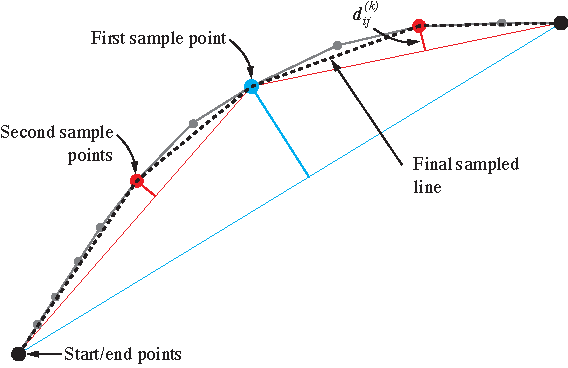
\includegraphics[scale=1]{rdp_illustration.pdf}
    \caption{RDP algorithm process. Starts by sampling the end points, then recursively sampling the point with maximum perpendicular distance between each set of sample points. Stops when the maximum perpendicular distance is less than the tolerance.}
    \label{fig:rdp-algo}
\end{figure}

\subsubsection{A related approach: Limiting global error}

Both the max deviation downsampler and the RDP algorithm operate using a local tolerance, $\epsilon$.
However, it may be more appropriate to use a global tolerance on the difference between sampled and original data.
The downsampled data can be compared with the original data using our ``standard'' error metric:
\begin{equation}
    \tilde{\varphi} = \sqrt{\frac{\int (\sigma_{test} - \sigma_{ds})^2 \dd \varepsilon^*}{E_{orig}}},
\end{equation}
where $E_{orig}$ is the total accumulated squared strain energy in the original data, $\sigma_{test}, \sigma_{ds}$ are the stress signals of the original and downsampled data, and $\varepsilon^*$ is the accumulated strain.
The definition of $\tilde{\varphi}$ is similar to that of $\bar{\varphi}$ from \citet{deCastroeSousaConsistencySolvingInverse2020} but simplified to a single test.
Linear interpolation is used to compute the downsampled data at each point between the sampled points, and the integrals are computed using the trapezoidal rule.

An algorithm to keep the error metric below a global tolerance, $\epsilon_g$ is provided in Algorithm~\ref{alg:global-err-downsampling}.
The idea is to select an initial (``large'') local tolerance, $\epsilon_0$.
Then reduce the local tolerance and re-run the downsampling until $\tilde{\varphi} < \epsilon_{g}$.
This always converges because the error is zero at the limit of sampling all the points.
This procedure is made accessible by the highly efficient implementation of the RDP algorithm in the Python package \texttt{polyprox}, however, the same process can be applied using other downsampling methods with a bit of time.
Note that my implementation uses the filtered/scaled ``$\sigma_{test}$'' to compute $\tilde{\varphi}$, thus, the true error between the sampled data tends to be slightly higher.

\begin{algorithm}
	\caption{Downsampling based on global energy error.}
	\label{alg:global-err-downsampling}
	\begin{algorithmic}[1]
		\State \textbf{input:} Set of points, $\{x_i\}_{i=0}^{N-1}$ with $x_i \in \mathbb{R}^n$ and $N \in \mathbb{Z}$; initial local tolerance, $\epsilon_0 \in \mathbb{R}$; and
        global tolerance $\epsilon_g \in \mathbb{R}$.
        \State \textbf{output:} Set of indices between $[0, N)$ to keep, $k_{sample}$.
        \State $\chi \gets 1.05$
        \Comment Factor to accelerate convergence
        \State $n_g \gets 10$
        \Comment Maximum number of iterations
        \State $i \gets 0$
        \State $\tilde{\varphi} \gets 10 \cdot \epsilon_g$
        \Comment Just to be larger than $\epsilon_g$ initially
        \State $\epsilon \gets \epsilon_0$
		\While{$\tilde{\varphi} > \epsilon_g$ and $i < n_g$}
            \State $k_{sample} \gets$ indices from downsampling with local tolerance $\epsilon$
            \State $\tilde{\varphi} \gets$ error metric computed using $\{x_i\}$ and $k_{sample}$
            \If{$\tilde{\varphi} > \epsilon_g$}
                \State $\epsilon \gets \epsilon \cdot (\epsilon_g / (\chi \, \tilde{\varphi}))$
                \State $i \gets i + 1$
            \EndIf
		\EndWhile
\end{algorithmic}
\end{algorithm}

\subsection{Additional sampling in the initial elastic region}

The initial elastic region is assumed to be bounded by the first point in the data and the upper yield point obtained in part 1 of the overall procedure.
It is important to have a few points in this region to obtain a good estimate of the initial elastic properties from the downsampled data.
Therefore, $n_{elastic}$, additional points are sampled in the initial elastic region at approximately evenly spaced strain intervals.
Each additional point is sampled using
\begin{equation}
    j = \arg \min \abs{x_i - x_{t}},
\end{equation}
where $x_t$ are the target evenly spaced strain points.

\subsection{Saturation in constant amplitude tests}

Cyclic hardening saturates logarithmically under constant amplitude cyclic loading in structural steel materials.
Therefore, many cycles may be associated with a small increase in stress and a large portion of data is associated with a small amount of information.
One option to reduce this data is to cut the cycles after saturation has been reached.
The saturation point is defined herein as the index of the first peak $i$ that satisfies $\sigma_i > \eta \cdot \max \sigma$ in the positive loading direction and $\sigma_i < \eta \cdot \min \sigma$ in the negative loading direction, with $0 < \eta \leq 1$.
The data after the saturation point is not sampled.

Cutting cycles after saturation in constant amplitude tests requires the definition of the saturation tolerance, $\eta$.
The minimum number of cycles to include, $n_{cyc}$, is also specified.


\subsection{Overall procedure}

The overall procedure is summarized in Algorithm~\ref{alg:overall-summary}.
The procedure consists of the two main and auxillary parts outlined earlier.
The original stress-strain data input to the procedure is $X = \{x_i \}_{i=0}^{N-1}$.
Algorithm~\ref{alg:overall-summary} produces a set of indices, $k_{sample}$.
The downsampled stress-strain data is $X_{ds} = \{ x_i \mid i \in k_{sample} \}$.
I emphasize that the downsampled data is sampled directly from the original data, therefore, $X_{ds} \subset X$.
(Just to emphasize that the filtered, normalized data is only used to determine the indices and the added elastic points are the closest indices to the targets.)
The global error method can be used instead by swapping line~\ref{algline:downsampler} with the results from Algorithm~\ref{alg:global-err-downsampling}.

I recommend using the following input parameters in Algorithm~\ref{alg:overall-summary}:
\begin{itemize}
    \item $f_{yn}$: based on the material
    \item $\eta = 0.99$
    \item $n_{cyc} = 20$
    \item if local method: $\epsilon = 0.001$
    \item if global method: $\epsilon_0 = 0.1$, $\epsilon_g = 0.005$
    \item $w = 5$
    \item $\alpha = 11$
    \item $p = 1$
    \item $n_{elastic} = 7$
\end{itemize}
The parameter $\eta = 0.99$ was selected as being close to 1.0 and $n_{cyc} = 20$ was selected from \citet{deCastroeSousaConsistencySolvingInverse2020} because at least 20 cycles are indicated.
Two window lengths are required for pre- and post-2~\% strain due to the different strain rates.
A value of $w = 5$ provides a weighted average of $\pm2$ points, and $\alpha = 11$ was selected because, even though the strain rate is around 26 times lower, the window length lead to too much aliasing in the pre-2~\% region with larger values.
Linear interpolation ($p = 1$) is recommended because it is most effective at reducing the noise.
The trade-off is that linear interpolation increase aliasing around peaks, however, the peaks are already included in part~1.
Seven additional points are added to the initial elastic region to give nine points total (seven + start + upper yield).
This should give 4--5 points in the $0.65 f_{yn}$ region used to compute the initial elastic modulus.
The $\epsilon, \epsilon_g$ recommendations were selected through trial and error to see when the stress-strain graphs became visually similar.


\begin{algorithm}
	\caption{Overall summary of the proposed downsampling method.}
	\label{alg:overall-summary}
	\begin{algorithmic}[1]
        \State \textbf{input data:} set of stress-strain data, $\{x_i\}_{i=0}^{N-1}$
        \State \textbf{input parameters:} nominal yield stress, $f_{yn}$; saturation tolerance in constant amplitude loading, $\eta$; minimum cycles in constant amplitude loading, $n_{cyc}$; downsampler tolerance(s), $\epsilon$ or $\epsilon_0, \epsilon_g$; filter window length post-2~\% strain, $w$; filter window length pre-2~\% factor, $\alpha$; filter interpolation order, $p$; number of additional points in the initial elastic region, $n_{elastic}$.

        \State \textbf{output:} $k_{sample}$ the indices of the sampled points.
        \bigskip

        \State Compute the initial elastic modulus and initial 0.2~\% offset yield stress using the nominal yield stress, $f_{yn}$
        \State $k_{1} \gets $ indices of the peaks in the stress-strain graph
        \If{constant amplitude loading}
            \State Determine $n_{sat}$ cycles to reach $\sigma_i > \eta \cdot \max \sigma$ and $\sigma_i < \eta \cdot \min \sigma$
            \If{$n_{sat} < n_{cyc}$}
                \State $n_{sat} \gets n_{cyc}$
            \EndIf
            \State Truncate data past $n_{sat}$ cycles
        \EndIf
        \State Filter stress data pre-2~\% strain with window length $\alpha \cdot w$ and order $p$
        \State Filter stress data post-2~\% strain with window length $w$ and order $p$
        \State Normalize the stress-strain data
        \State $k_2 \gets$ indices from downsampler with local ($\epsilon$) or global method ($\epsilon_g, \epsilon_0$) \label{algline:downsampler}
        \State $k_3 \gets$ indices of $n_{elastic}$ evenly spaced points in the initial elastic region
        \State $k_{sample} \gets k_1 \cup k_2 \cup k_3$
    \end{algorithmic}
\end{algorithm}



\section{Results}

Detailed results from the HEM320 web and S235/275 15~mm plate datasets are provided in this section to comment on certain aspects of downsampling stress-strain data.
The results shown in this section were computed using the recommended parameters for the global-error downsampling method using the RDP algorithm.
Typical downsampled results are compared with original data in Figure~\ref{fig:sampled-compare-dots}.

The error metrics for the ten load protocols and reduction factors are provided in Figure~\ref{fig:error-and-reduction}.
The error metric, $\tilde{\varphi}$, is computed using $k_{sample}$ from the proposed global downsampling method.
The $\tilde{\varphi}$ values are computed using the ``true'' original data (i.e., not filtered and not normalized), this is why they may be larger than 0.5~\%.
The average value for the HEM320 web dataset is 0.514~\% and for the S235/275 dataset is 0.558~\%.
The error metric is not computed for the integer reduction method because I did not save the indices.
A more detailed comparison of the different methods in terms of resulting stress-strain is provided for one example in Figure~\ref{fig:hem320-lp8-compare-methods}.

The reduction factors are the number of points in the original divided by the number of samples in the downsampled data.
Reduction factors are provided for the proposed (New) and integer reduction (Old) downsampling methods.
The values are not computed for the old method in LPs 4 and~5 because cycle cutting is not employed.
The total number of data points for all LPs are reduced by 75.8 times for the HEM320 web and 90.0 times for the S235/275.
Neglecting LPs 4 and 5, the new method reduces the total number of data points by 2.6 times compared to the old method for the HEM320 web and 5.7 times for the S235/275.


\begin{figure}
    \centering
    \begin{subfigure}[b]{0.49\linewidth}
        \centering
        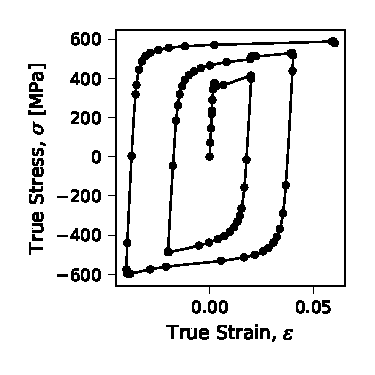
\includegraphics{LP8_dots_WP3_HEM320_C_CRM20.pdf}
        \caption{HEM320 web}
        \label{fig:hem320-lp8-results}
    \end{subfigure}
    \begin{subfigure}[b]{0.49\linewidth}
        \centering
        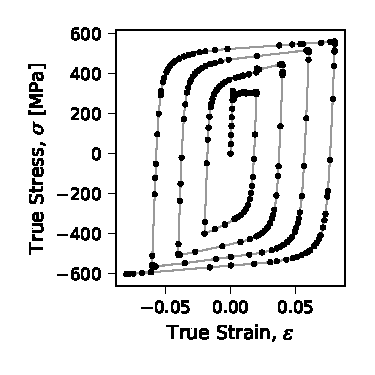
\includegraphics{LP8_dots_S235275_Plate15.pdf}
        \caption{S235/275 15~mm plate}
        \label{fig:s235275-lp8-results}
    \end{subfigure}
    \caption{Sampled points in LP8 from datasets. Line is the original data, dots are the sampled points using the proposed method.}
    \label{fig:sampled-compare-dots}
\end{figure}


\begin{figure}
    \centering
    \begin{subfigure}[b]{0.45\linewidth}
        \centering
        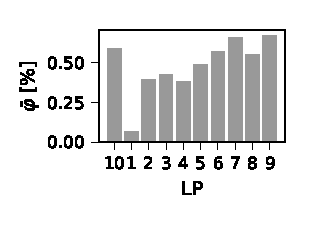
\includegraphics{error_WP3_HEM320_C_CRM20.pdf}
        \caption{Error, HEM320 web}
        \label{fig:hem320-error}
    \end{subfigure}
    \begin{subfigure}[b]{0.45\linewidth}
        \centering
        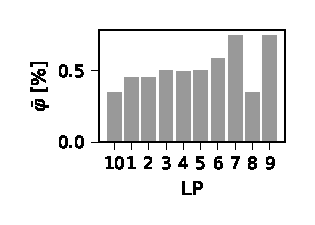
\includegraphics{error_S235275_Plate15.pdf}
        \caption{Error, S235/275 15~mm plate}
        \label{fig:s235275-error}
    \end{subfigure}

    \begin{subfigure}[b]{0.45\linewidth}
        \centering
        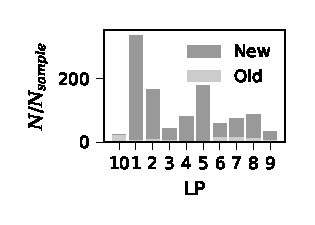
\includegraphics{N_reduction_WP3_HEM320_C_CRM20.pdf}
        \caption{Reduction, HEM320 web}
        \label{fig:hem320-reduction}
    \end{subfigure}
    \begin{subfigure}[b]{0.45\linewidth}
        \centering
        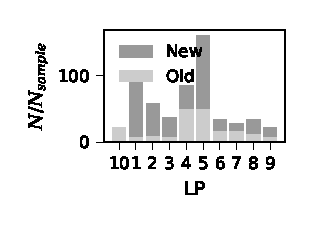
\includegraphics{N_reduction_S235275_Plate15.pdf}
        \caption{Reduction, S235/275 15~mm plate}
        \label{fig:s235275-reduction}
    \end{subfigure}
    \caption{Error and Reduction factors between original and downsampled data. New is the proposed method, Old is the integer factor downsampling.}
    \label{fig:error-and-reduction}
\end{figure}


\begin{figure}
    \centering
    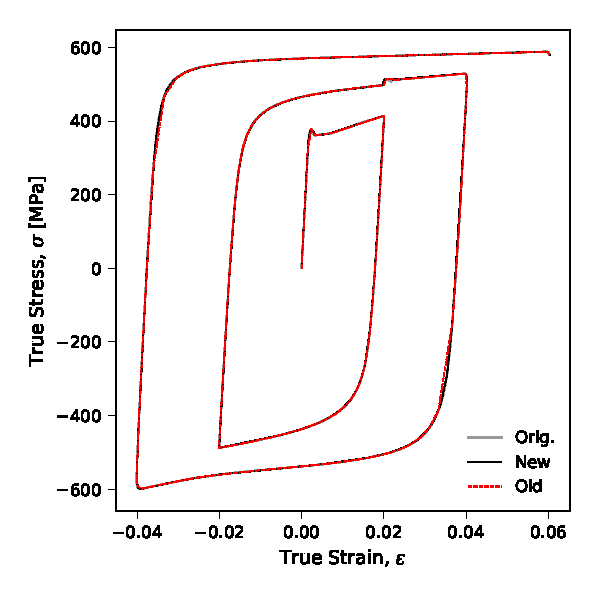
\includegraphics{LP8_WP3_HEM320_C_CRM20.pdf}
    \caption{Comparison of different methods for downsampling LP8 in the HEM320 web dataset. New is the proposed method, Old is the integer factor downsampling.}
    \label{fig:hem320-lp8-compare-methods}
\end{figure}


\section{Discussion}

\subsection{Evaluation of results}

Figure~\ref{fig:sampled-compare-dots} shows that the sampled points tend to be concentrated in the regions of high curvature and the initial elastic region.
Additionally, the peaks of the stress-strain graph are all sampled.
Using the global method, the procedure is straightforward and interpretable.
Figures~\ref{fig:hem320-error} and~\ref{fig:s235275-error} show that the error with the global method is around 0.5~\%.
At this level of error, the data is reduced by between 50--90 times compared to the original.

The main strengths of the global error method are its reliability and its relation to the inverse problem in \citet{deCastroeSousaConsistencySolvingInverse2020}.
For example, the old method does not sample the curved parts of the graph in Figure~\ref{fig:hem320-lp8-compare-methods} as well as the new method.
This is despite having multiple times more points for the same graph (see Figure~\ref{fig:hem320-reduction}).
The global method allows an analyst to decide on an acceptable downsampling tolerance with relation to the inverse problem of material calibration.
For instance, $\tilde{\varphi} = 0.5$~\% is approximately one order of magnitude lower than the values of $\bar{\varphi}$ expected in VC/UVC calibration \citep{deCastroeSousaConsistencySolvingInverse2020}.
Therefore, the downsampling process is expected to have a fairly limited impact on the minimization of $\varphi$ defined in \citet{deCastroeSousaConsistencySolvingInverse2020}.
A stricter tolerance can be specified depending on the application and requirements of the analyst.

Another strength of the RDP method is that it is strain rate independent because it is based on the curvature of the data and will sample points appropriately.
However, the strain rate leads to the main difficultly in the proposed downsampling method, which is the choice of filtering parameters.
The recommended $w$ and $\alpha$ parameters appear to work well as long as the standard load protocols are followed, however, different values are certainly required for different strain and sampling rates.
My implementation of Algorithm~\ref{alg:overall-summary} in \texttt{rlmtp} (RESSLab Material Test Processing) uses the default values set forth above, and also allows users to modify all of these parameters.
The input parameters for tests that do not follow the standard load protocols can be saved in a file and read by the algorithm when the downsampling occurs.

\subsection{Choice of algorithm}

The choice between the maximum deviation downsampler and RDP algorithms is discussed in this section.
The max deviation downsampler is not recommended for two reasons:
(i) it has higher errors because it does not guarantee the maximum perpendicular distance is always less than the tolerance, and (ii) my implementation in Python is slow compared to the RDP algorithm in \texttt{polyprox}.
The first issue being more critical, of course.
The first issue is rooted in the nature of our data having many inflection points.
With multiple inflection points, although $d^{(k)}_{ij} < \epsilon$, there may be some $d^{(l)}_{mj} > \epsilon$ with $m > i$ and $m < l < j$.
Therefore, ``stepping forward'', as in the maximum deviation downsampler, is not as good of a strategy as used in the RDP algorithm.
The max deviation downsampler tends to produce higher errors in terms of $\tilde{\varphi}$ for the same $\epsilon$ (although it results in less points).
This makes the second issue not worth investigating, although it could likely be fixed by implementing the max deviation downsampler in C as is done with the RDP algorithm in \texttt{polyprox}.

With regards to the RDP algorithm, the cyclic nature of our stress-strain data implies that selecting the start and end points, then sampling the maximum perpendicular distance between these, is not a great heuristic.
See Figure~\ref{fig:rdp-algo}.
This is because the maximum perpendicular distance from the line linking the start and end points is not necessarily at a region of high curvature.
However, the RDP algorithm is not optimal in producing the minimum number of points, but it will be on the ``safe side'' of adding a few additional points to get the job done.
The results could be more efficient (i.e., satisfy the local $\epsilon$ criteria with less points) by using an optimal solution from \citet{ChanApproximationPolygonalCurves1996}.
The RDP implementation be made more time efficient (particularly for the global method) considering \citet{HershbergerSpeedingDouglasPeuckerLineSimpli1992}.
However, Algorithm~\ref{alg:global-err-downsampling} can already be run on the most extensive load protocols in a few seconds using \texttt{polyprox}.

\subsection{Different distance measures}

A challenge in the max deviation downsampler and RDP methods is the difference in units between stress and strain.
I currently overcome this challenge by re-scaling the stress-strain data, then using the 2-norm when computing the perpendicular distance.
Options that could be used rather than rescaling the data are:
\begin{enumerate}
    \item use the angle between the line and each point,
    \item use the norm induced by an alternative inner product: $\norm{d_k}_S = \sqrt{d_k \cdot S \cdot d_k}$, and
    \item use an energy criterion.
\end{enumerate}

The first option is similar to the maximum perpendicular distance, but more sensitive to noise.
This is because of the small angle rule, $\sin \theta \approx \theta$, and the perpendicular distance is $\norm{v}_2 \sin \theta$, where $v = x_k - x_i$.
If $\norm{v}_2$ is small, the angle can have a large variation (i.e., in the case of high frequency noise), however, the perpendicular distance remains small.

In the second option, Algorithm~\ref{alg:max-dev-downsampler} remains essential the same except for how $d^{(k)}_{ij}$ is computed.
To use a matrix-vector notation:
\begin{equation*}
    d^{(k)}_{ij} = \begin{bmatrix}
        (d^{(k)}_{ij})_{\varepsilon} \\
        (d^{(k)}_{ij})_{\sigma}
    \end{bmatrix}, \quad
    S = \begin{bmatrix}
        \frac{1}{(\max \varepsilon - \min \varepsilon)^2} & 0 \\
        0 & \frac{1}{(\max \sigma - \min \sigma)^2}
    \end{bmatrix},
\end{equation*}
where the values of $S$ would in this case give a similar effect to the scaling that I already use.
Other options for $S$ could be selected.
Essentially, we compute a scaled distance rather than scale the data itself.
This method would still require a selection of tolerance $\epsilon$, but it may be different depending on the matrix $S$.

In the third option, the perpendicular distance criterion is replaced by the energy bounded by the polygon.
In this case, instead of $d_k$'s we compute
\begin{equation*}
    e = \int_{\varepsilon_i}^{\varepsilon_j} (\sigma - l_\sigma) \dd \varepsilon,
\end{equation*}
where $l_\sigma$ represents the stress signal of the line between $x_i$ and $x_j$.
If the stress-strain graph is nearly straight, then $(\sigma - l_\sigma) \approx 0$.
The point $j-1$ would be sampled if $e > \epsilon$.

The benefits of the second method are that it does not require any scaling of the data and the error is closely related to the calibration problem.
However, the link between the energy, $e$, and the curvature in the stress-strain graph is less clear, making it more difficult to reason about an appropriate tolerance.
Everything considered, a tolerance still needs to be selected regardless of the method.
I went with the data scaling option because, in my opinion, the link between the algorithm and the geometric interpretation of curvature is most clear.
Furthermore, this makes the overall procedure more easily adapted to existing algorithms (e.g., \texttt{polyprox}).

\subsection{More than two dimensions}

This document assumes two-dimensional data parametrized as a function of time, i.e., $x(t) \in \mathcal{D} \times \mathcal{T}$, where $\mathcal{D} \subset \mathbb{R}^n$ and $n$ is the dimension of the data ($n = 2$ in our case---uniaxial stress/strain), and $t \in \mathcal{T}$ is the time.
Algorithm~\ref{alg:overall-summary} can easily be extended to $n > 2$ by preserving curvature in each considered data pair.
The same procedure can then be used with an appropriate tolerance, $\epsilon$, and an appropriate scaling procedure by sampling a point anytime the tolerance is exceeded by one of the pairs.
Considering higher dimensions may be useful, for instance:
\begin{itemize}
    \item when downsampling temperature and stress-strain data together (can preserve curvature in both temperature-strain and stress-stress), and
    \item when downsampling data considering multiple components of the stress-strain tensor (e.g., multiaxial material tests).
\end{itemize}


\section{Conclusion}

Integer reduction downsampling is not efficient for the stress-strain data that we collect for material tests.
A better downsampling procedure was proposed in Algorithm~\ref{alg:overall-summary} consisting of two main steps and two auxiliary steps.
The main steps are (i) to determine the peaks of the stress-strain graph and (ii) to then use a downsampling algorithm that preserves the curvature in the stress-strain graph.
The maximum deviation downsampler and Ramer–Douglas–Peucker (RDP) algorithms were considered in (ii).
A global-error preserving method was proposed because these algorithms operate on a local criterion.
The auxillary steps are to add points to the initial elastic region and to remove cycles after saturation of cyclic hardening in constant amplitude tests.
Heuristic parameters applicable to tests carried out according to the standard load protocols were provided.
Results from two datasets were provided to indicate the performance of the proposed method.
The main conclusions are:
\begin{itemize}
    \item Re-scaling the stress and strain signals prior to downsampling is suggested to mimic the geometric notion of curvature in stress-strain graphs. A scaled distance could be computed instead, however, this seems to be more complicated than just scaling the data. An acceptable local error, $\epsilon$, has to be selected regardless of this choice.
    \item The RDP algorithm is better than the maximum deviation downsampler because it is more strict in enforcing the local tolerance and it is faster.
    \item The RDP algorithm leads to satisfactory results as a curvature-preserving downsampler. It is not the optimal solution to the min-\# problem and results may be slightly improved with an optimal algorithm.
    \item Filtering the stress signal is necessary to get the best performance out of downsamplers, however, this adds a complication regarding the selection of filter parameters.
    \item The global error method (Algorithm~\ref{alg:global-err-downsampling}) is recommended because of its link with material calibration problems.
    \item Using the proposed method, the number of data points is reduced by one to two orders of magnitude based on the examined datasets. This reduction was around 2--5 times better than the integer reduction method. The proposed method appears to provide to a better representation of stress-strain data with fewer points.
\end{itemize}


\bibliographystyle{unsrtnat}
\bibliography{ds_references}

\end{document}
